% Unofficial UChicago CS Poster Template
% v1.1.0 released September 8, 2022
% https://github.com/k4rtik/uchicago-poster
% a fork of https://github.com/anishathalye/gemini

\documentclass[final]{beamer}

% ====================
% Packages
% ====================

\usepackage[T1]{fontenc}
\usepackage{lmodern}
\usepackage[size=custom,width=127,height=106.68,scale=1.15]{beamerposter}
\usetheme{gemini}
\usecolortheme{uchicago}
\usepackage{graphicx}
\usepackage{booktabs}
\usepackage{doi}
\usepackage[labelfont=bf]{caption}
\usepackage[numbers]{natbib}
\usepackage[patch=none]{microtype}
\usepackage{tikz}
\usepackage{pgfplots}
\pgfplotsset{compat=1.18}
\usepackage{anyfontsize}
\usepackage{textgreek}
\pdfstringdefDisableCommands{%
\def\translate#1{#1}%
}

\graphicspath{ {./img/} }
% ====================
% Lengths
% ====================

% If you have N columns, choose \sepwidth and \colwidth such that
% (N+1)*\sepwidth + N*\colwidth = \paperwidth
\newlength{\sepwidth}
\newlength{\colwidth}
\setlength{\sepwidth}{0.025\paperwidth}
\setlength{\colwidth}{0.3\paperwidth}

\newcommand{\separatorcolumn}{\begin{column}{\sepwidth}\end{column}}

% ====================
% Title
% ====================

\title{Single Molecule Mechanics and Kinetics of Cardiac Myosin Interacting with Regulated Thin Filaments}

\author{Brent Scott \inst{1} \and Sarah R. Clippinger Schulte  \inst{1} \and Samantha K. Barrick \inst{1} \and W. Tom Stump \inst{1} \and Tommy Blackwell \inst{1} \and Michael J. Greenberg \inst{1}}

\institute[shortinst]{\inst{1} Biochemistry and Molecular Biophysics, Washington University in St. Louis}

% ====================
% Footer (optional)
% ====================

\footercontent{
  \href{https://glab.biochem.wustl.edu/}{https://glab.biochem.wustl.edu/}
   \hfill
   2023 Annual Biophysical Society Meeting
   \hfill
  \href{mailto:brents@wustl.edu}{brents@wustl.edu}}
% (can be left out to remove footer)

% ====================
% Logo (optional)
% ====================

% use this to include logos on the left and/or right side of the header:
% \logoright{\includegraphics[height=7cm]{logo1.pdf}}
% \logoleft{\includegraphics[height=7cm]{logo2.pdf}}

% ====================
% Body
% ====================

\begin{document}
\addtobeamertemplate{headline}{}
{
    \begin{tikzpicture}[remember picture,overlay]
      \node [anchor=north west, inner sep=3cm] at ([xshift=0.0cm,yshift=1.2cm]current page.north west)
      {
\includegraphics[height=5.0cm]{logos/washu-logo.jpg}}; % also try shield-white.eps
      \node [anchor=north east, inner sep=3cm] at ([xshift=0.5cm,yshift=1.3cm]current page.north east)
      {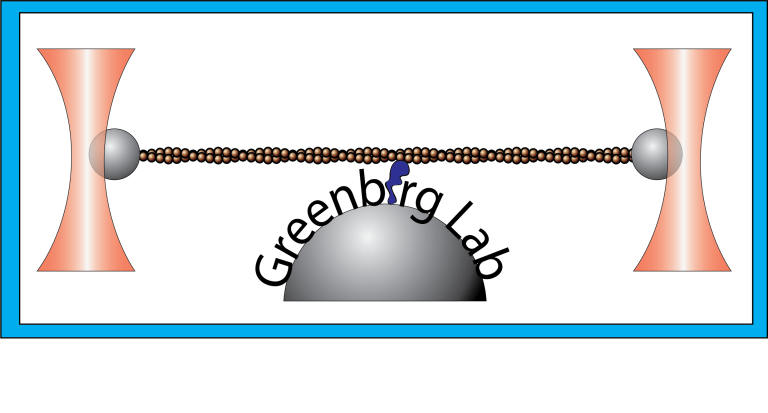
\includegraphics[height=6.0cm]{logos/greenberg-lab-logo.png}};
    \end{tikzpicture}
}

\begin{frame}[t]
\begin{columns}[t]
\separatorcolumn

\begin{column}{\colwidth}
  \begin{block}{Cardiac myosin powers the heart}
    % \begin{minipage}{0.48 \textwidth}
    \begin{center}
      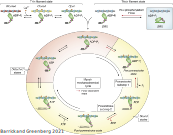
\includegraphics[scale=1.65]{barrick-greenberg-xb}
      \end{center}
    %   \end{minipage}
    %   \begin{minipage}{0.48 \textwidth}
        \textbf{The power produced by the heart to pump blood is generated by cardiac myosin} pulling on thin filaments. \textbf{This process is highly regulated} through the regulatory proteins \textbf{troponin (Tn)} and \textbf{tropomyosin (Tm)} that wrap around actin filaments in the sarcomere to form the thin filament. Many \textit{in vitro} investigations into cardiac myosin's mechanics and kinetics have been performed with actin in the absence of the regulatory proteins, and these characterizations provide fundamental information into the mechanisms underlying contraction of the heart. \textbf{Despite the central roles that Tn/Tm have in the regulation of force generation in the heart, their effects on cardiac myosin's mechanics are not well understood.}
      %\end{minipage}
  \end{block}


  \begin{block}{Regulatory proteins can affect myosin's function}
    Characterizing cardiac myosin's mechanics and kinetics in the presence of Tn/Tm is important since similiar \textbf{studies conducted with other myosins show that regulatory proteins can alter myosin's behavior on actin:}
    \begin{itemize}
      \item \textbf{Tm 4.2 increases the force sensitivity} of non-muscle myosin II (Hundt et al. 2016)
      \item \textbf{Myosin-V (Myo2p) only walks processively in the presence of Tm} due to a slowing of myosin's ADP release rate (Hodges et al. 2012)
      \item \textbf{Regulatory proteins reduce skeletal myosin's unitary step size} and slow detachment from actin (Kad et al. 2005)
      \item Conversely, the \textbf{regulatory proteins have no effect on skeletal myosin's step size across a range of [Ca\textsuperscript{2+}]}, but decrease myosin's attachment rate to actin (Longyear et al. 2017)
    \end{itemize}
  \end{block}

  \begin{block}{Our Approach}
    We investigated the effects of regulated thin filaments on cardiac myosin's mechanics and kinetics using:
    \begin{enumerate}
      \item \textbf{Optical tweezers} (schematic shown below) to measure the magnitudes and rates underlying myosin's two mechanical substeps and the attachment duration to the thin filament at \textbf{low (1~{\textmu}M) ATP}
      \item An \textbf{isometric force clamp} to measure the load-dependence of cardiac myosin's mechanics and kinetics at a \textbf{physiological relevant 1 mM ATP}
    \item \textbf{Stopped flow kinetics} to measure the rates of ADP release and ATP-induced actomyosin dissociation
  \end{enumerate}
   \centering \includegraphics[scale=2.3]{traps-cardiac-sm}
  \end{block}

\end{column}

\separatorcolumn

\begin{column}{\colwidth}

  \begin{alertblock}{Significance Statement}

    While excellent studies have elucidated the mechanics and kinetics underlying the interactions between cardiac myosin and actin at the single molecule scale, the majority of these studies have been conducted in the absence of regulatory proteins. In the case of several other myosin isoforms, regulatory proteins alter the mechanics and load-dependent kinetics of myosin's working stroke; \textbf{however, it is not clear what role, if any thin filament regulatory proteins play in tuning the cardiac myosin working stroke and load-dependent kinetics.}

  \end{alertblock}

  \begin{block}{Critical Controls}
    \begin{figure}
      
\includegraphics[scale=0.6]{motility-controls}
      \caption{To ensure that the incorporation of biotin-actin into polymerized filaments necessary for the optical trapping experiments would not disrupt regulation of actin by Tn/Tm, control experiments were performed. \textbf{a)} An optical trapping trace shows no binding events were observeable at low Ca\textsuperscript{2+} with regulated thin filaments. \textbf{b)} At high Ca\textsuperscript{2+}, frequent myosin binding events occur with regulated thin filaments. \textbf{c)} Data from \textit{in vitro} motility shows that myosin moved bare actin and biotin-actin thin filaments at similiar velocities at pCa 4 and stopped all movement at pCa 9 demonstrating \textbf{Tn/Tm can properly regulate biotin-actin filaments.}}
    \end{figure}

    \end{block}

    \begin{block}{\large{Single molecule mechanics of {\textbeta}-cardiac myosin (1~{\textmu}M ATP)    }}
      \begin{figure}
         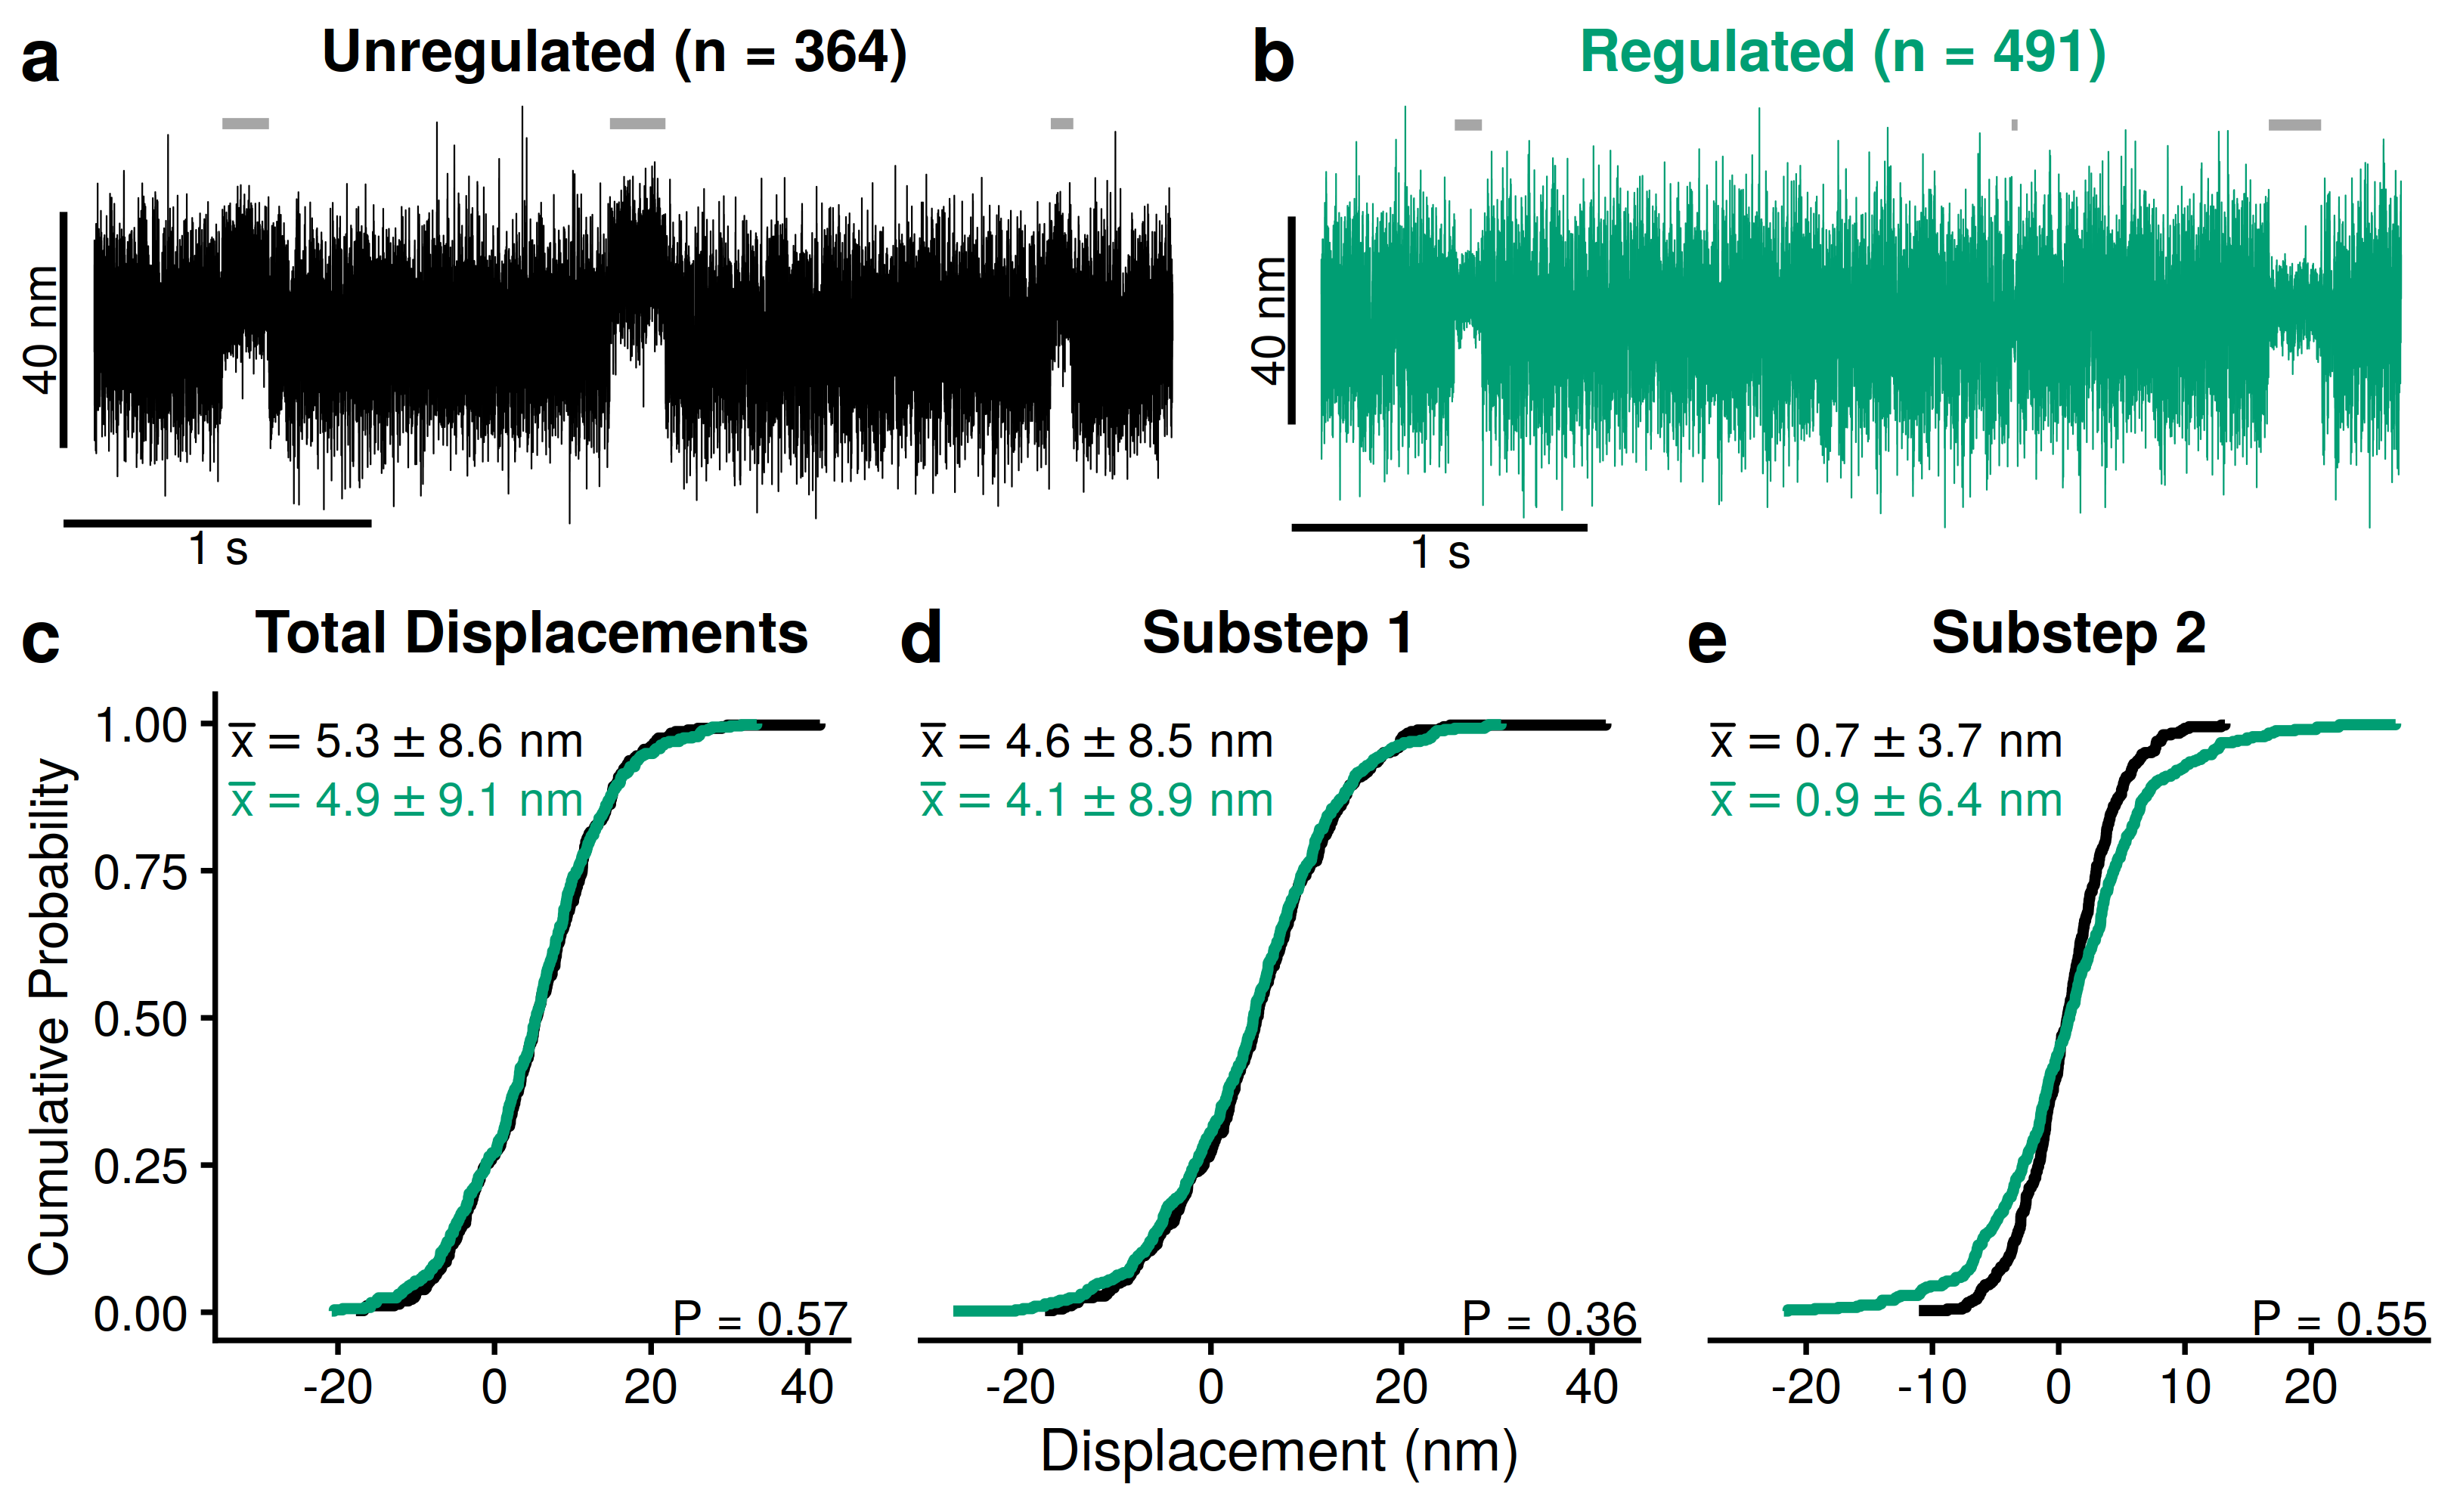
\includegraphics[scale=1.8]{step-size}
         \caption{\textbf{a)} Optical trapping traces for an unregulated actin filament (black) and \textbf{b)} regulated thin filament (green) at pCa 4, low ATP (1~{\textmu}M). Myosin actin interactions are highlighted with gray horizontal markers. Cumulative distributions of the \textbf{c)} total displacements, \textbf{d)} first, and \textbf{e)} second substep are shown. \textbf{There are no differences between cardiac myosin's mechanics as measured in the optical trap between unregulated and regulated conditions at 1~{\textmu}M ATP.}}

        \end{figure}
  \end{block}

  \begin{block}{Ensemble averages of the myosin working stroke}
      \begin{figure}
        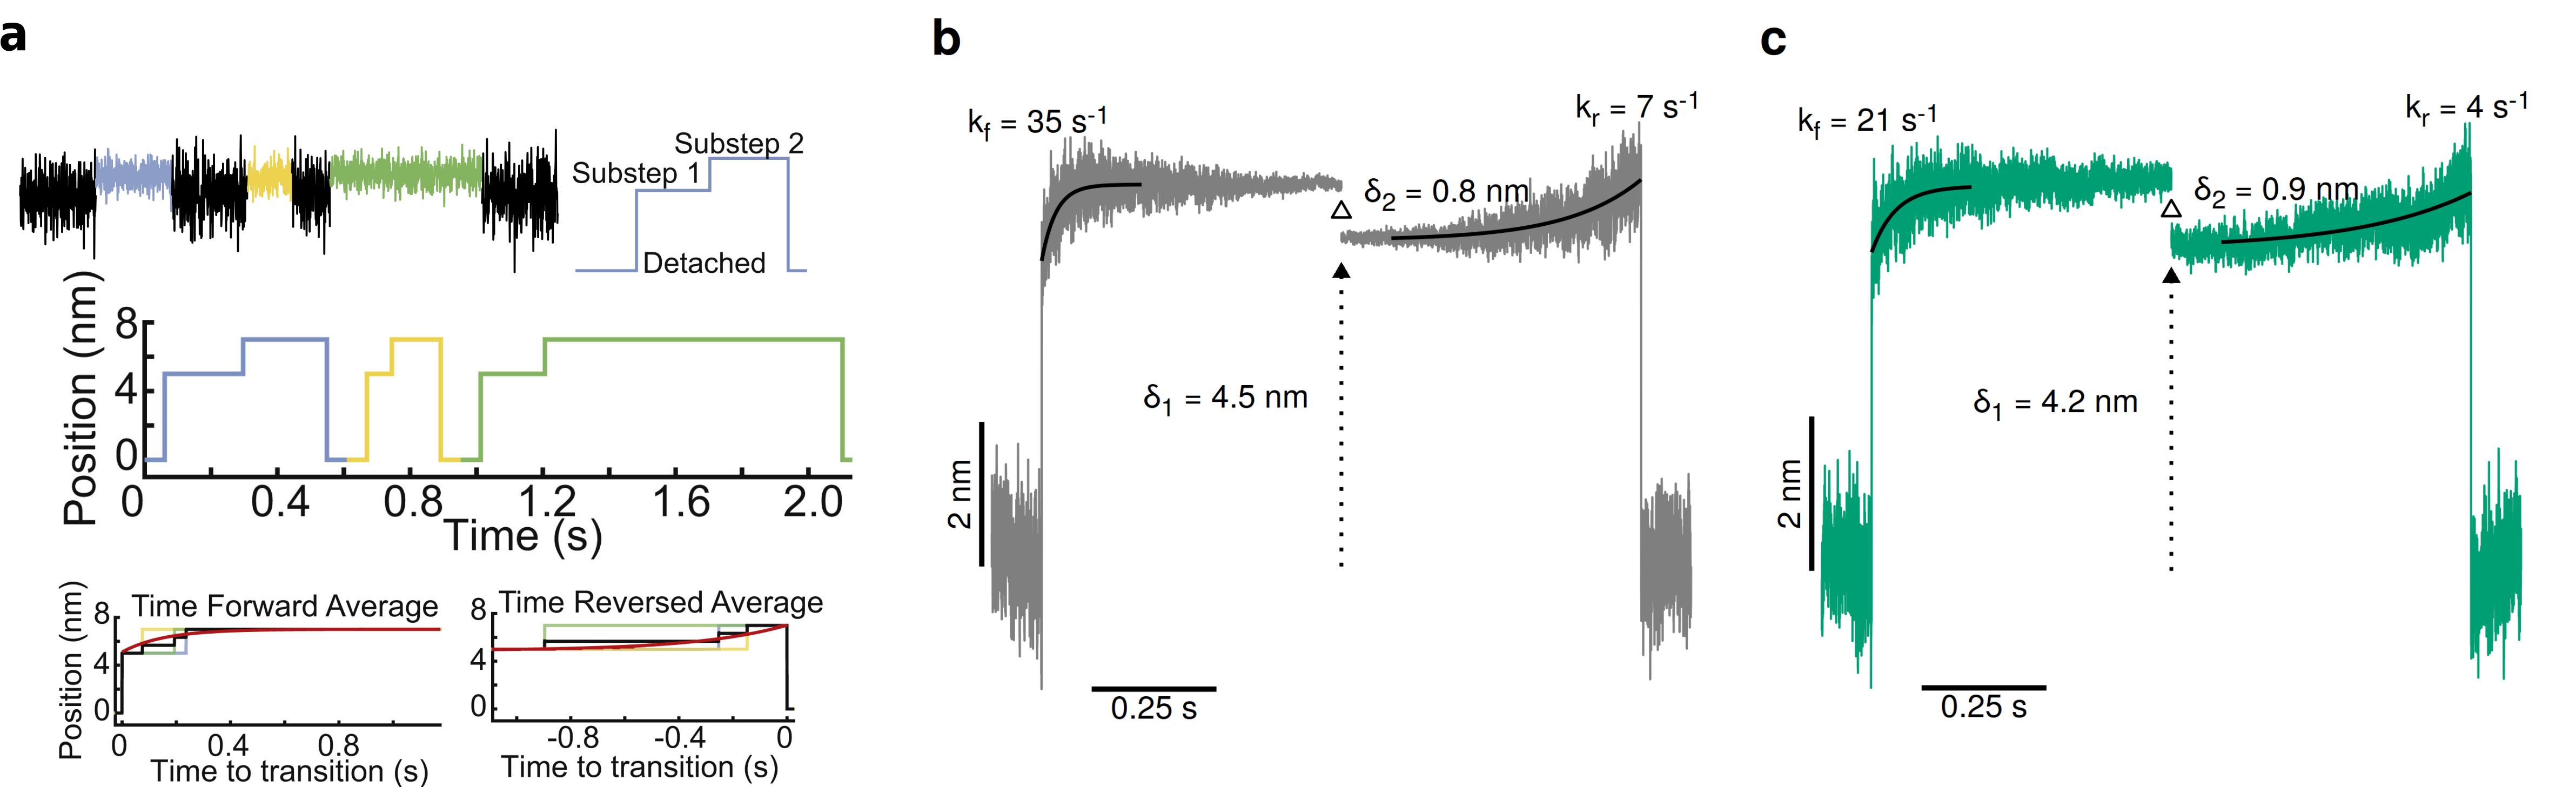
\includegraphics[scale=1.4]{ea-draw}
        \caption{Myosin's mechanical powerstroke occurs in two substeps. The first is rapid upon binding to actin and the second is slower and temporally associated with ADP release. \textbf{a)} The ensemble averages of single molecule binding interactions reveal the two distinct mechanical substeps and the associated rates by fitting a single exponential to data from \textbf{b)} unregulated and \textbf{c)} regulated actin filaments. $d_{1}$ and $d_{2}$ represent the size of the first and second working strokes (nm), and $k_{f}$ and $k_{r}$ are rates associated with ADP release and ATP-induced dissociation. \textbf{The ensemble averages show the magnitudes and rates of cardiac myosin's mechanical substeps are similiar between the unregulated and regulated conditions.}}
        \end{figure}
  \end{block}%


\end{column}

\separatorcolumn

\begin{column}{\colwidth}
  \begin{block}{Kinetics of actomyosin dissociation}

    \begin{minipage}{0.58 \textwidth}
      \begin{figure}
        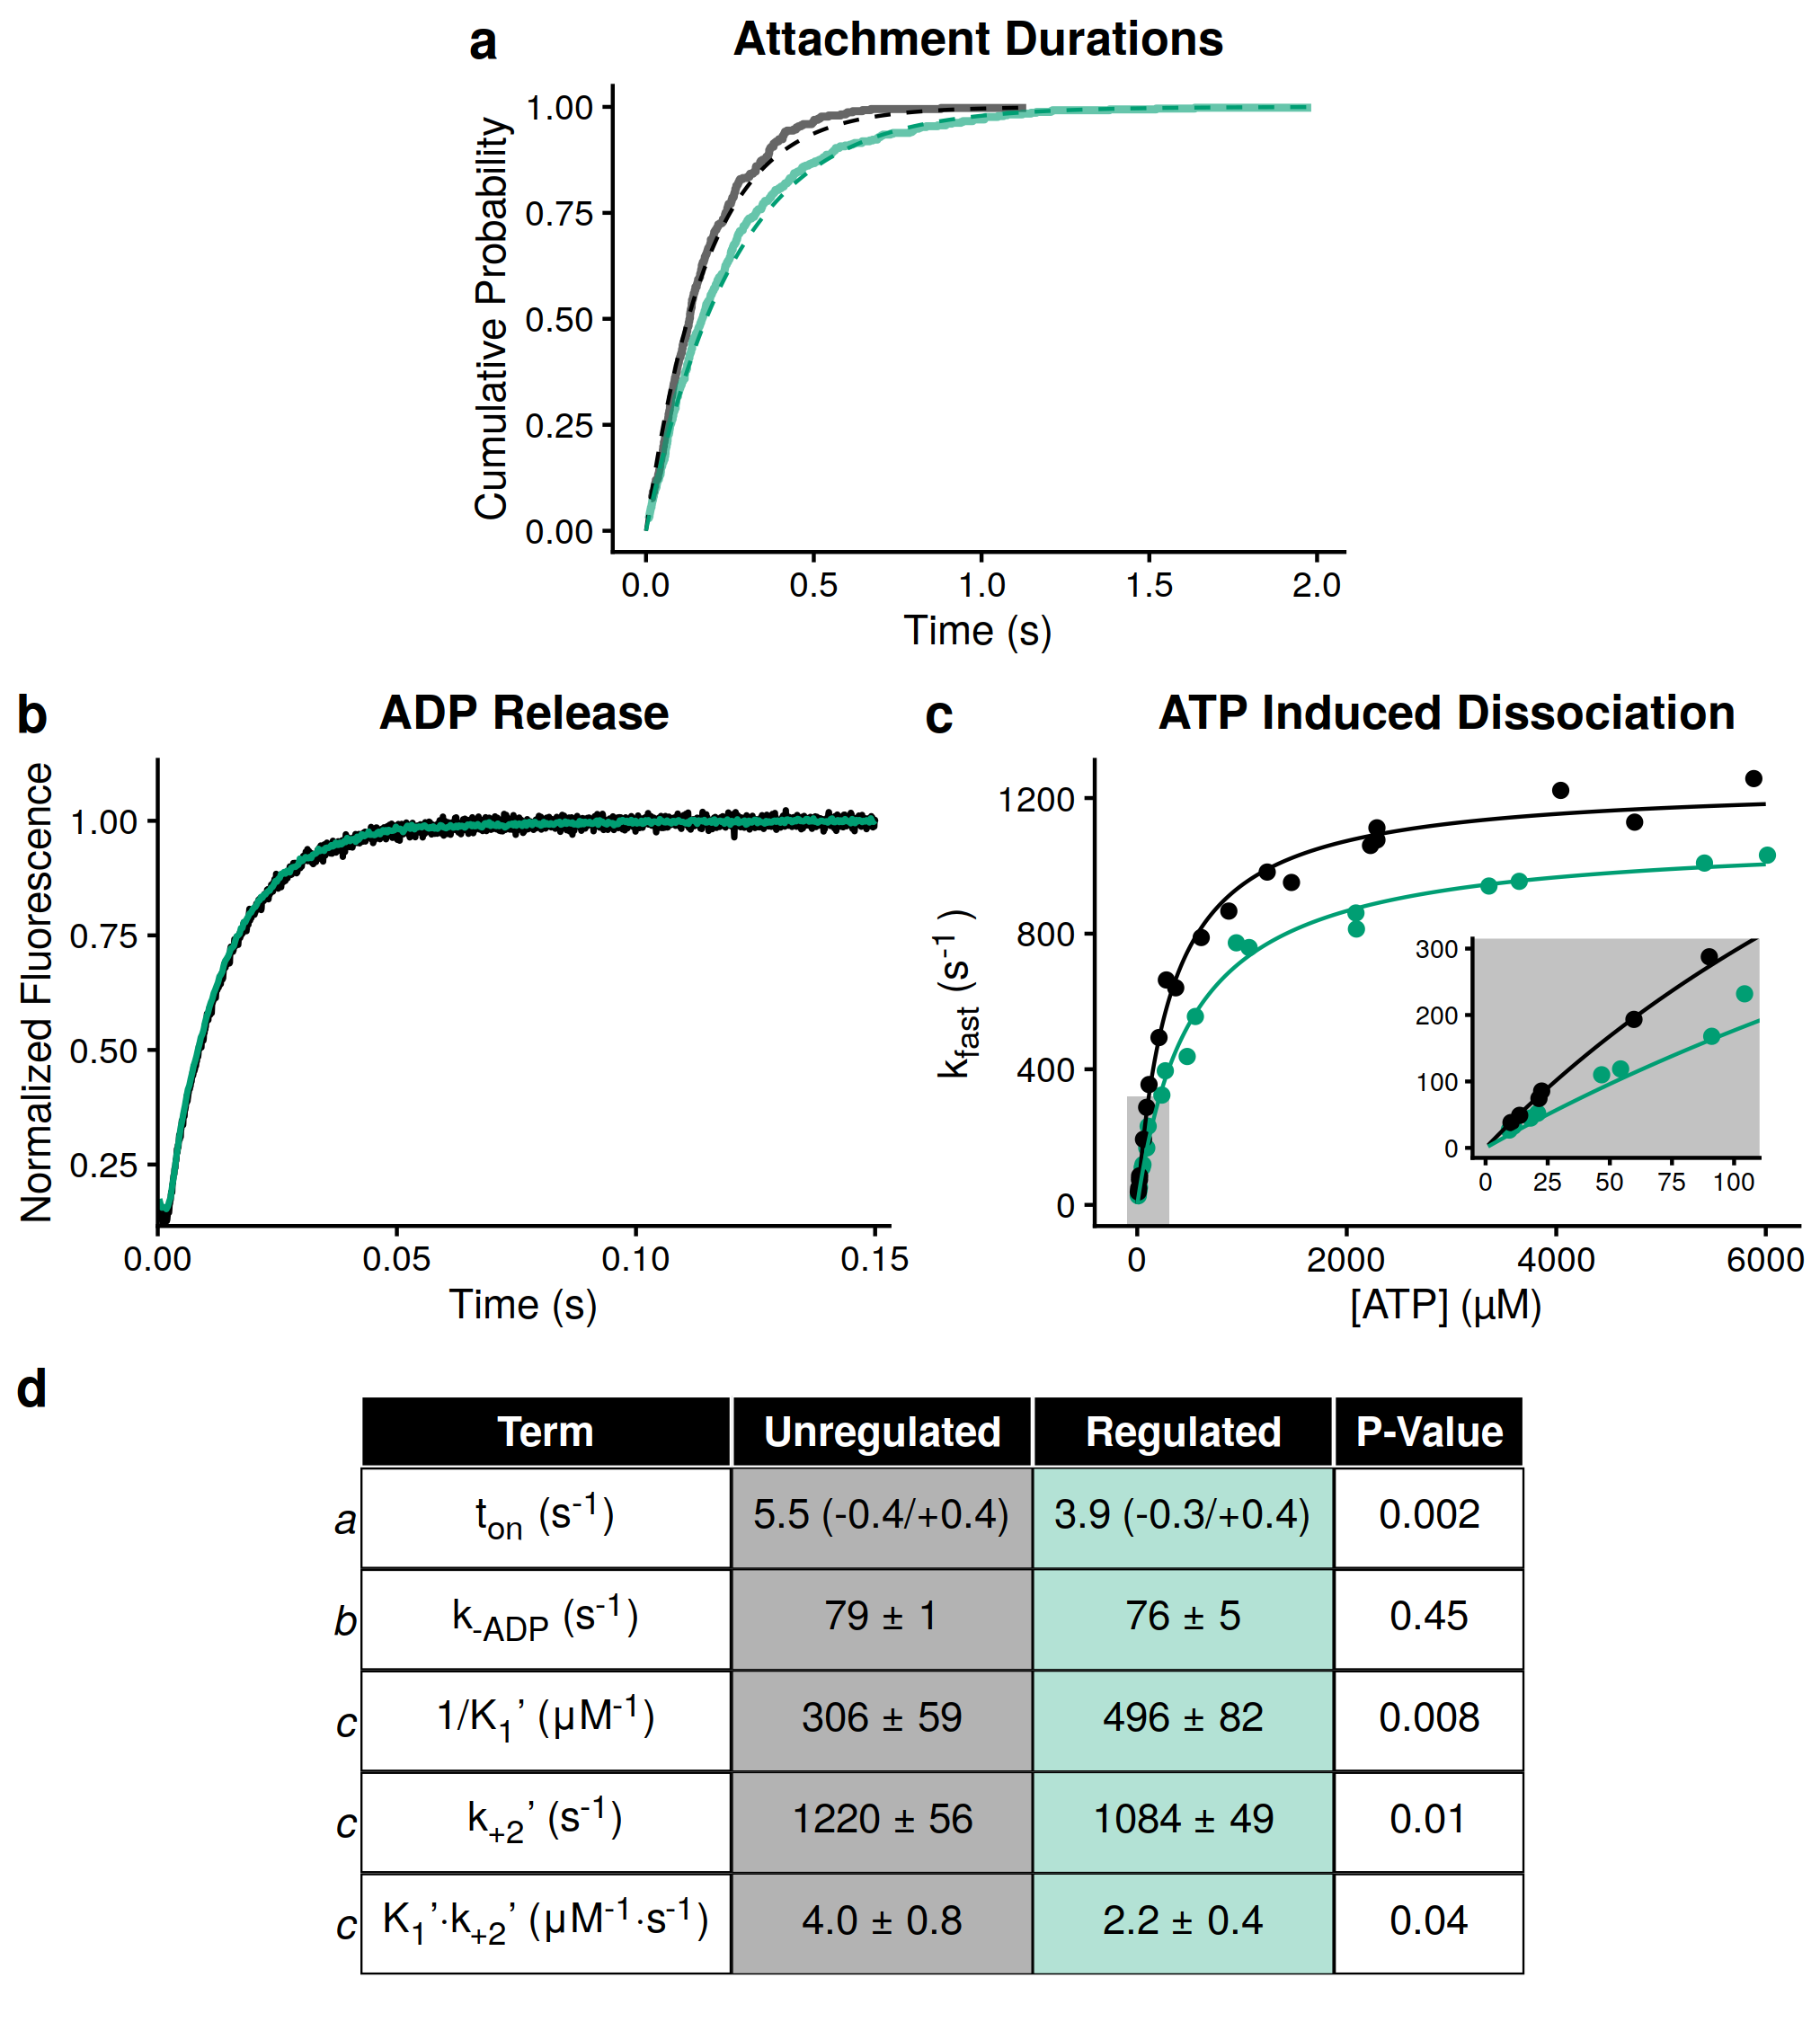
\includegraphics[scale=1.3]{figure-3_kinetics}
        \end{figure}
    \end{minipage}
    \begin{minipage}{0.38 \textwidth}
      \begin{figure}
        \caption{\textbf{a)} Cumulative distributions of the attachment durations from the optical trap show \textbf{cardiac myosin remained attached to thin filaments for longer durations than to bare actin filaments at low ATP} (1~{\textmu}M). \textbf{b)} Representative fluorescence transients measuring the rate of ADP release from actomyosin. Data is an average of 5 technical replicates. \textbf{There is no difference in the rate of ADP release} measured using unregulated or regulated thin filaments in stopped flow (pyrene-actin). \textbf{c)} ATP-induced dissociation curves (k\textsubscript{fast}) show \textbf{at low ATP, cardiac myosin has a slower second-order ATP-induced dissociation rate when interacting with regulated thin filaments.} \textbf{d)} Table of parameters obtained from all kinetic measurements. Row letter corresponds to the figure panel which the data is from. Row 'a' value is average and 95\% CI, and all others are the average +/- standard deviation.}
        \end{figure}
    \end{minipage}
  \end{block}

  \begin{block}{Load-dependence of myosin's kinetics at 1 mM ATP}
    \centering
    \begin{figure}
      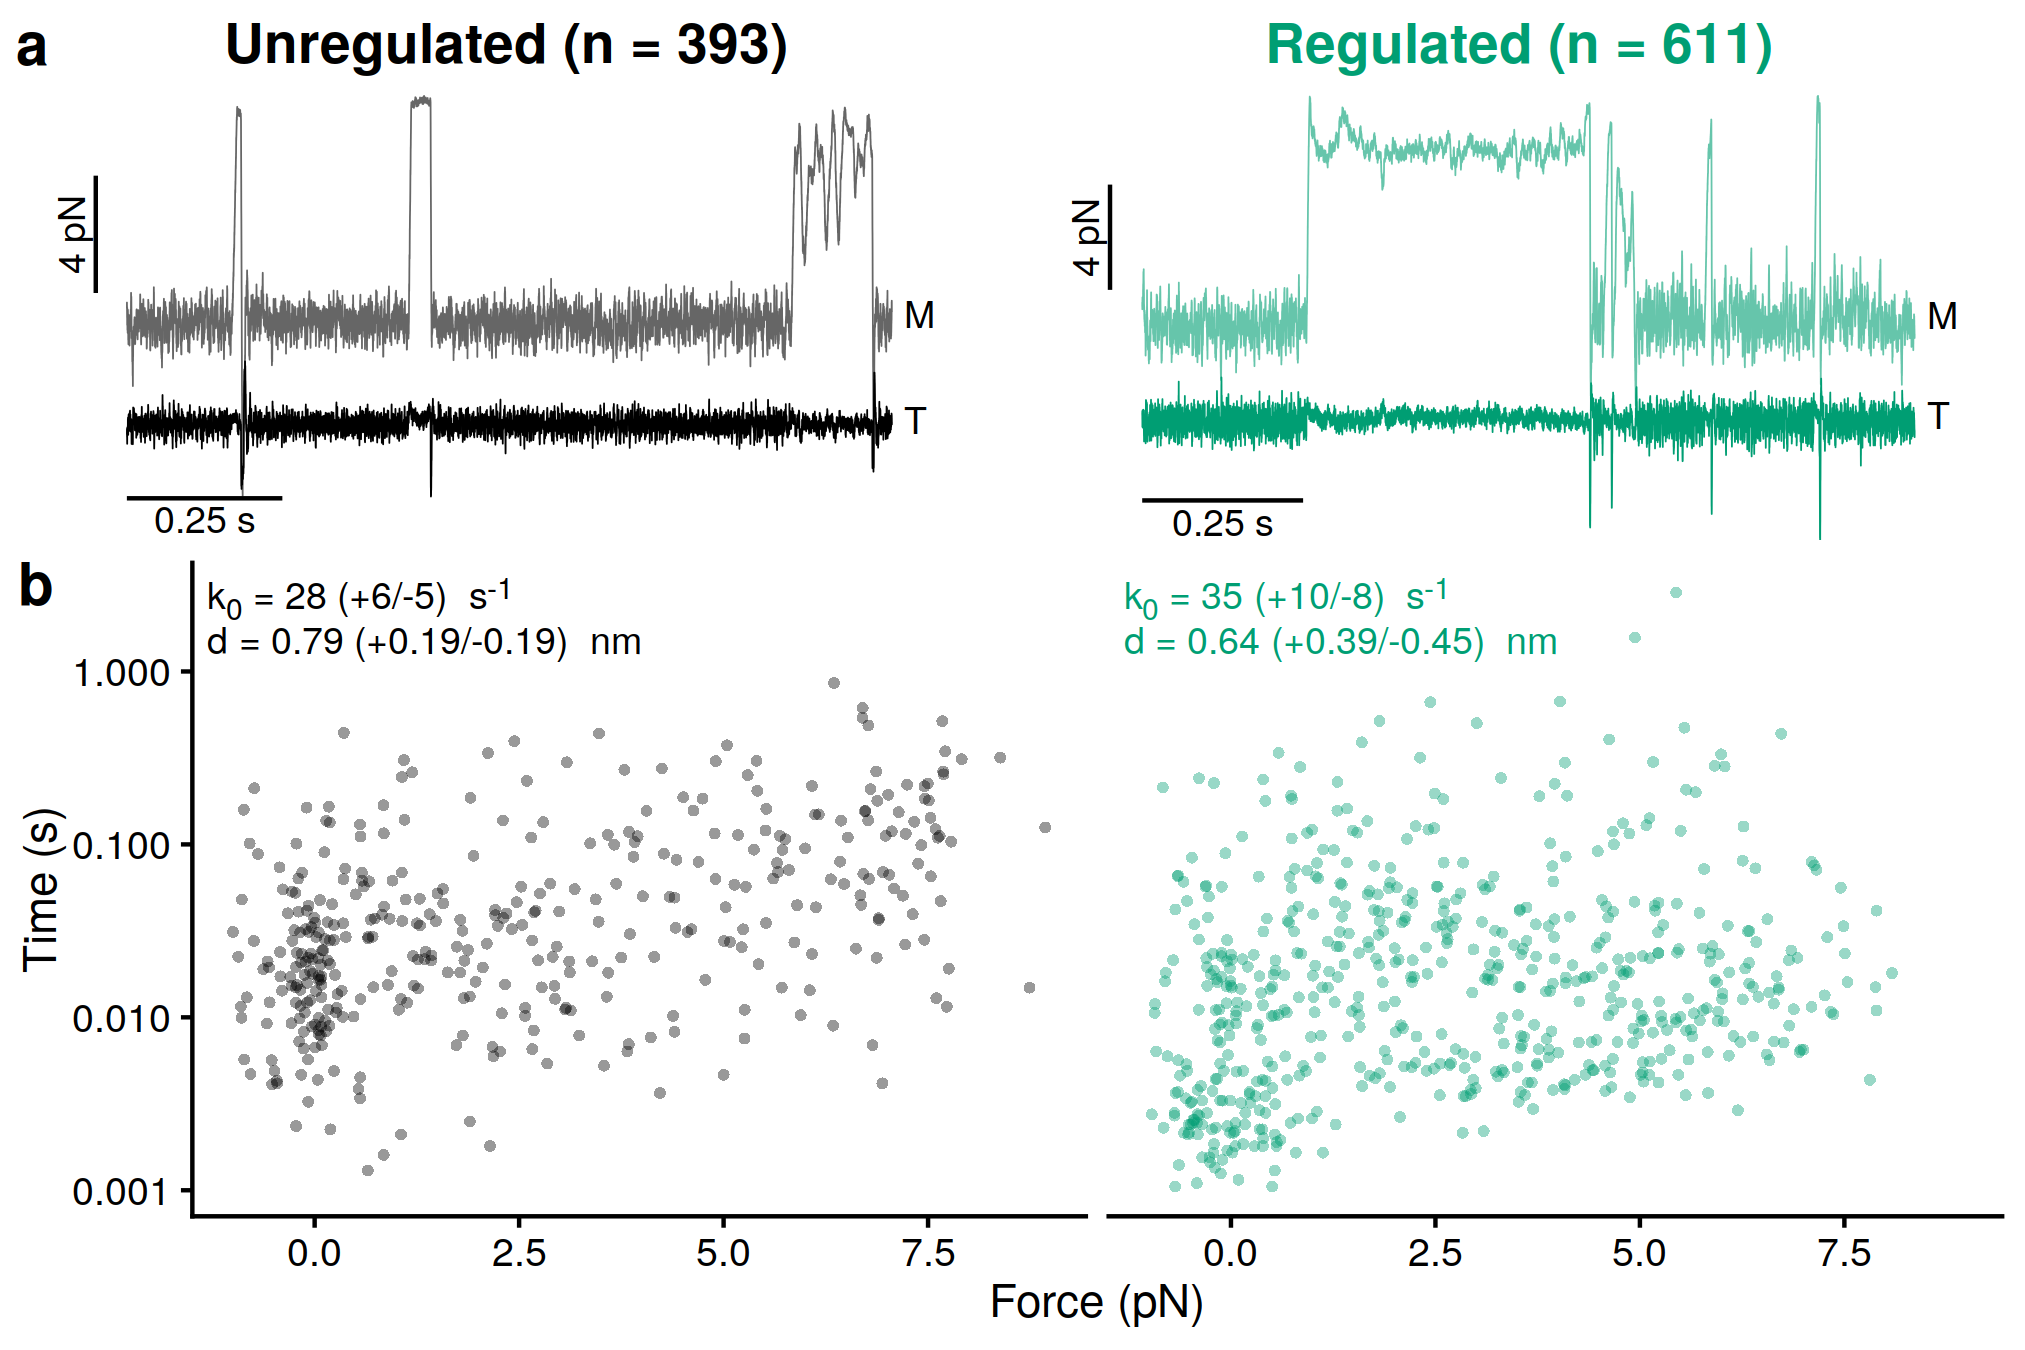
\includegraphics[width = 34cm]{figure-4_feedback}
      \caption{We used an isometric force clamp to measure the load-dependence of myosin's mechanics and kinetics at a \textbf{physiological relevant 1 mM ATP.} \textbf{a)} Data traces from the isometric force clamp are labeled 'M' or 'T' representing the motor or transducer beads. The position of the transducer bead is monitored and held isometric as corrections are applied to the motor bead. \textbf{b)} The resulting attachment durations versus force. The data were fitted with Bell's equation using maximum likelihood estimation. The parameter \textit{d} describes the load-dependent transition while $k_{0}$ represents the detachment rate in the absence of load. \textbf{The presence of the regulatory proteins on actin had no effects on the load-dependent measurements made with the force clamp at saturating ATP.}}
      \end{figure}
  \end{block}

  \begin{block}{Key Points}

    \begin{itemize}
      \item Both the magnitudes and rates of the two substeps of cardiac myosin's working stroke are not affected by regulatory proteins
      \item The load-dependence of cardiac myosin's mechanics and kinetics are unchanged by regulatory proteins
      \item At physiological ATP concentrations, there are no differences in the rates of ADP release or ATP-induced dissociation
      \item Interestingly at low ATP (1~{\textmu}M), we saw increased attachment durations in the presence of the regulatory proteins which coincided with a slowed second-order ATP-induced dissociation rate measured using stopped flow. This suggests that regulatory proteins may act as more than just a simple steric block to regulate myosin binding at low ATP
    \end{itemize}

    \textbf{All together, the results suggest regulatory proteins do not affect cardiac myosin's mechanics or kinetics at physiological relevant ATP concentrations, which has important implications for future efforts to model muscle contraction and heart disease.}

    \vspace{5mm}

    \tiny{This work was supported by the National Institutes of Health (R01 HL141086 to M.J.G.) and the Children’s Discovery Institute of Washington University and St. Louis Children’s Hospital (PM-LI-2019-829 to M.J.G.)}
  \end{block}
\end{column}

\separatorcolumn
\end{columns}
\end{frame}

\end{document}

%%% Local Variables:
%%% coding: utf-8
%%% mode: latex
%%% TeX-engine: luatex
%%% TeX-master: t
